\documentclass[]{article}
\usepackage{lmodern}
\usepackage{amssymb,amsmath}
\usepackage{float}
\usepackage{ifxetex,ifluatex}
\usepackage{fixltx2e} % provides \textsubscript
\ifnum 0\ifxetex 1\fi\ifluatex 1\fi=0 % if pdftex
  \usepackage[T1]{fontenc}
  \usepackage[utf8]{inputenc}
\else % if luatex or xelatex
  \ifxetex
    \usepackage{mathspec}
  \else
    \usepackage{fontspec}
  \fi
  \defaultfontfeatures{Ligatures=TeX,Scale=MatchLowercase}
\fi
% use upquote if available, for straight quotes in verbatim environments
\IfFileExists{upquote.sty}{\usepackage{upquote}}{}
% use microtype if available
\IfFileExists{microtype.sty}{%
\usepackage{microtype}
\UseMicrotypeSet[protrusion]{basicmath} % disable protrusion for tt fonts
}{}
\usepackage[margin=1in]{geometry}
\usepackage{hyperref}
\hypersetup{unicode=true,
            pdftitle={Assignment 3},
            pdfauthor={Terry Liu},
            pdfborder={0 0 0},
            breaklinks=true}
\urlstyle{same}  % don't use monospace font for urls
\usepackage{color}
\usepackage{fancyvrb}
\newcommand{\VerbBar}{|}
\newcommand{\VERB}{\Verb[commandchars=\\\{\}]}
\DefineVerbatimEnvironment{Highlighting}{Verbatim}{commandchars=\\\{\}}
% Add ',fontsize=\small' for more characters per line
\usepackage{framed}
\definecolor{shadecolor}{RGB}{248,248,248}
\newenvironment{Shaded}{\begin{snugshade}}{\end{snugshade}}
\newcommand{\KeywordTok}[1]{\textcolor[rgb]{0.13,0.29,0.53}{\textbf{#1}}}
\newcommand{\DataTypeTok}[1]{\textcolor[rgb]{0.13,0.29,0.53}{#1}}
\newcommand{\DecValTok}[1]{\textcolor[rgb]{0.00,0.00,0.81}{#1}}
\newcommand{\BaseNTok}[1]{\textcolor[rgb]{0.00,0.00,0.81}{#1}}
\newcommand{\FloatTok}[1]{\textcolor[rgb]{0.00,0.00,0.81}{#1}}
\newcommand{\ConstantTok}[1]{\textcolor[rgb]{0.00,0.00,0.00}{#1}}
\newcommand{\CharTok}[1]{\textcolor[rgb]{0.31,0.60,0.02}{#1}}
\newcommand{\SpecialCharTok}[1]{\textcolor[rgb]{0.00,0.00,0.00}{#1}}
\newcommand{\StringTok}[1]{\textcolor[rgb]{0.31,0.60,0.02}{#1}}
\newcommand{\VerbatimStringTok}[1]{\textcolor[rgb]{0.31,0.60,0.02}{#1}}
\newcommand{\SpecialStringTok}[1]{\textcolor[rgb]{0.31,0.60,0.02}{#1}}
\newcommand{\ImportTok}[1]{#1}
\newcommand{\CommentTok}[1]{\textcolor[rgb]{0.56,0.35,0.01}{\textit{#1}}}
\newcommand{\DocumentationTok}[1]{\textcolor[rgb]{0.56,0.35,0.01}{\textbf{\textit{#1}}}}
\newcommand{\AnnotationTok}[1]{\textcolor[rgb]{0.56,0.35,0.01}{\textbf{\textit{#1}}}}
\newcommand{\CommentVarTok}[1]{\textcolor[rgb]{0.56,0.35,0.01}{\textbf{\textit{#1}}}}
\newcommand{\OtherTok}[1]{\textcolor[rgb]{0.56,0.35,0.01}{#1}}
\newcommand{\FunctionTok}[1]{\textcolor[rgb]{0.00,0.00,0.00}{#1}}
\newcommand{\VariableTok}[1]{\textcolor[rgb]{0.00,0.00,0.00}{#1}}
\newcommand{\ControlFlowTok}[1]{\textcolor[rgb]{0.13,0.29,0.53}{\textbf{#1}}}
\newcommand{\OperatorTok}[1]{\textcolor[rgb]{0.81,0.36,0.00}{\textbf{#1}}}
\newcommand{\BuiltInTok}[1]{#1}
\newcommand{\ExtensionTok}[1]{#1}
\newcommand{\PreprocessorTok}[1]{\textcolor[rgb]{0.56,0.35,0.01}{\textit{#1}}}
\newcommand{\AttributeTok}[1]{\textcolor[rgb]{0.77,0.63,0.00}{#1}}
\newcommand{\RegionMarkerTok}[1]{#1}
\newcommand{\InformationTok}[1]{\textcolor[rgb]{0.56,0.35,0.01}{\textbf{\textit{#1}}}}
\newcommand{\WarningTok}[1]{\textcolor[rgb]{0.56,0.35,0.01}{\textbf{\textit{#1}}}}
\newcommand{\AlertTok}[1]{\textcolor[rgb]{0.94,0.16,0.16}{#1}}
\newcommand{\ErrorTok}[1]{\textcolor[rgb]{0.64,0.00,0.00}{\textbf{#1}}}
\newcommand{\NormalTok}[1]{#1}
\usepackage{longtable,booktabs}
\usepackage{graphicx,grffile}
\usepackage{graphicx}
\makeatletter
\def\maxwidth{\ifdim\Gin@nat@width>\linewidth\linewidth\else\Gin@nat@width\fi}
\def\maxheight{\ifdim\Gin@nat@height>\textheight\textheight\else\Gin@nat@height\fi}
\makeatother
% Scale images if necessary, so that they will not overflow the page
% margins by default, and it is still possible to overwrite the defaults
% using explicit options in \includegraphics[width, height, ...]{}
\setkeys{Gin}{width=\maxwidth,height=\maxheight,keepaspectratio}
\IfFileExists{parskip.sty}{%
\usepackage{parskip}
}{% else
\setlength{\parindent}{0pt}
\setlength{\parskip}{6pt plus 2pt minus 1pt}
}
\setlength{\emergencystretch}{3em}  % prevent overfull lines
\providecommand{\tightlist}{%
  \setlength{\itemsep}{0pt}\setlength{\parskip}{0pt}}
\setcounter{secnumdepth}{0}
% Redefines (sub)paragraphs to behave more like sections
\ifx\paragraph\undefined\else
\let\oldparagraph\paragraph
\renewcommand{\paragraph}[1]{\oldparagraph{#1}\mbox{}}
\fi
\ifx\subparagraph\undefined\else
\let\oldsubparagraph\subparagraph
\renewcommand{\subparagraph}[1]{\oldsubparagraph{#1}\mbox{}}
\fi

%%% Use protect on footnotes to avoid problems with footnotes in titles
\let\rmarkdownfootnote\footnote%
\def\footnote{\protect\rmarkdownfootnote}

%%% Change title format to be more compact
\usepackage{titling}

% Create subtitle command for use in maketitle
\newcommand{\subtitle}[1]{
  \posttitle{
    \begin{center}\large#1\end{center}
    }
}

\setlength{\droptitle}{-2em}

  \title{Assignment 3}
    \pretitle{\vspace{\droptitle}\centering\huge}
  \posttitle{\par}
    \author{Terry Liu 1630005038}
    \preauthor{\centering\large\emph}
  \postauthor{\par}
    \date{}
    \predate{}\postdate{}


\begin{document}
\maketitle


\subsection{Answer on Question One}\label{answer-one}


(a) \ Since the prior distribution is  Dirichlet distribution, the posterior distribution is also the Dirichlet distribution: $p(\theta|y) = \text{ Dirichelet } (y_1 + a_1 + \dots + y_n + a_n)$. From the properties of of the Dirichlet distribution, the marginal posterior distribution of $(\theta_1, \theta_2, 1 - \theta_1 - \theta_2)$ is also Dirichlet:

$$p(\theta_1, \theta_2 | y) \propoto theta_1^{y_1 + a_2 - 1} \theta_2^{y_2 + a_2 - 1} ( 1 - \theta_1 - \theta_2)^{y_{rest} + a_{rest} - 1}, \text{ where } y_{rest} = y_3 + \dots + y_J, a_{rest} = a_3 + \dots + a_J.$$

We can do a change of the varialbes to $(\alpha, \beta) = (\frac{\theta_1}{\theta_1 + \theta_2}, \theta_1 + \theta_2$. The Jacobian of this tranformation is $\begin{bmatrix} \frac{1}{\beta}\end{bmatrix}$, so the transformed density is :

$\begin{align*}
p(\alpha, \beta|y) &\propoto \beta(\alpha \beta)^{y_1 + a_1 -1}((1 - \alpha)^{y_2 + \alpha_2 - 1})(1 - \beta)^{y_{rest}= + \alpha_{rest} -1} \\
&= \alpha^{y_1 - a_1 -1}(1 - \alpha)^{y_2 + \alpha_2 -1} \beta^{y_1 + y_2 + \alpha_1 + \alpha_2 - 1} (1 - \beta)^{y_{rest} + \alpha_{rest} - 1} \\
&\propoto \text{Beta}(\alpha|y_1  + \alpha_1, y_2 + a_2) \text{Beta}(\beta|y_1 + y_2 + a_1 + a_2, y_{rest} + a_{rest})
\end{align*}$

Since the posterior density divides into separate factors for $\alpha$  and $\beta$, they are independent, so the posterior distribution is $\alph|y~text{ Beta } (y_1 + a_1, y_2, a_2)$.

(b) \ The \ $\text{Beta} (y_1 + a_1, y_2 + a_2)$ posterior distribution can also be derived from a $\text{Beta}(a_1, a_2}$ prior distribution and a binomial observation $y_1$ with sample size $y_1 + y_2$.

\subsection{Answer on Question Two}\label{answer-two}

Asume independent uniform prior distributions on he multinomial parameters. Then the posterior distributions are independent multinomial:

$\begin{align*}
(\pi_1, \pi_2, \pi_3)|y &\sim \text{Dirchlet}(295, 308, 39) \\
(\pi_1^*, \pi_2^*, \pi_3^*)|y &\sim \text{Dirchlet}(289, 333, 20)
\end{align*}$

and $\alpha_1 \frac{\pi_1}{\pi_1 + \pi_2}, \ \alpha_2 = \frac{\pi_1^*}{\pi_1^* + \pi_2^*}$. From the properties of the Dirichlet distribution:

$\begin{align*}
\alpha_1 | y \sim \text{ Beta }(295, 308) \\
\alpha_2 | y \sim \text{ Beta} (289, 333)
\end{align*}$

The histrogram of $2000$ draws from the posterior density of $\alph_2 - \alpha_1$ is attached, Based on this histogram, the posterior probability that there was a shift toward Bush is $19\%$

\begin{Verbatim}
alpha.1 <- rbeta (2000, 295, 308)
alpha.2 <- rbeta (2000, 289, 333)
dif <- alpha.2 - alpha.1
hist (dif, xlab="alpha_2 - alpha_1", yaxt="n",
  breaks=seq(-.12,.08,.01), cex=2)
print (mean(dif>0))
\end{Verbatim}

\begin{figure}[H]
  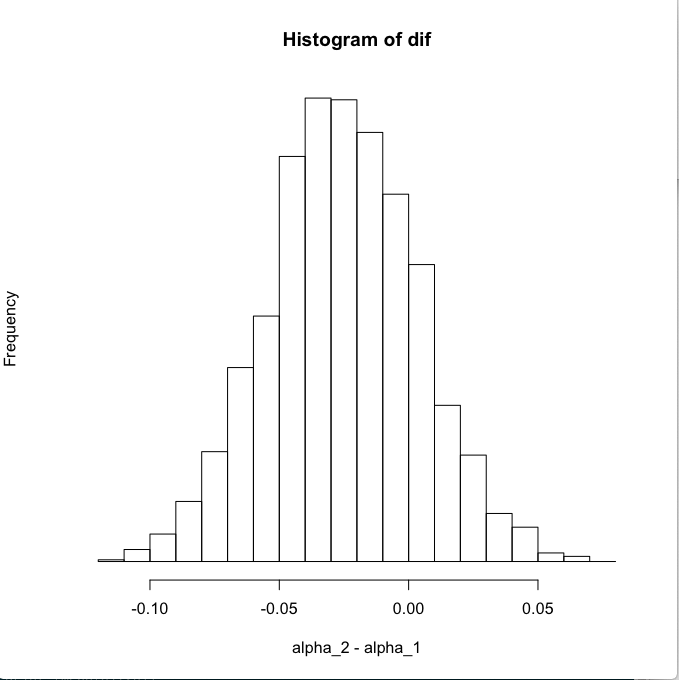
\includegraphics{question2.png}
  \caption{}
  \label{ histogram}
\end{figure}

\subsection{Answer of Question Three} \label{answer-3}

Data distribution is $p(y | \mu_c, \mu_t, \sigma_c, \sigma_t) = \prod_{i = 1}^32 N(y_{ci}\mu_c, \sigma_c^2) \prod_{i=1}^36 N(y_{yi}|\mu_t,\sigma_t^2).$ Posterior distribution is $p(y | \mu_c, \mu_t, log \sigma_c, log \sigma_t) = p(y | \mu_c, \mu_t, log \sigma_c, log \sigma_t)p(y|\mu_c, \mu_t, log \sigma_c, log \sigma_t))$

THe posteriror density fators, so $(\mu_c, \sigma_c)$ are independent of $(\mu_t, \sigma_t)$ in the posterior distribution. So, under this model, we can analyze the two experiments separately. We notice that the posterior distributions for $\mu_c$ and $\mu_t$ are:

$\begin{align*}
\mu_c|y \sim t_{31}(1.013, \farc{0.24^2}{32})\\
\mu_t|y \sim t_{35}(1.173, \farc{0.20^2}{36})
\end{align*}$

We can use R to print the plot:

\begin{Verbatim}
mu.c <- 1.013 + (0.24/sqrt(32))*rt(1000,31)
mu.t <- 1.173 + (0.20/sqrt(36))*rt(1000,35)
dif <- mu.t - mu.c
hist (dif, xlab="mu_t - mu_c", yaxt="n", breaks=seq(-.1,.4,.02), cex=2)
print (sort(dif)[c(25,976)])
\end{Verbatim}

\begin{figure}[H]
  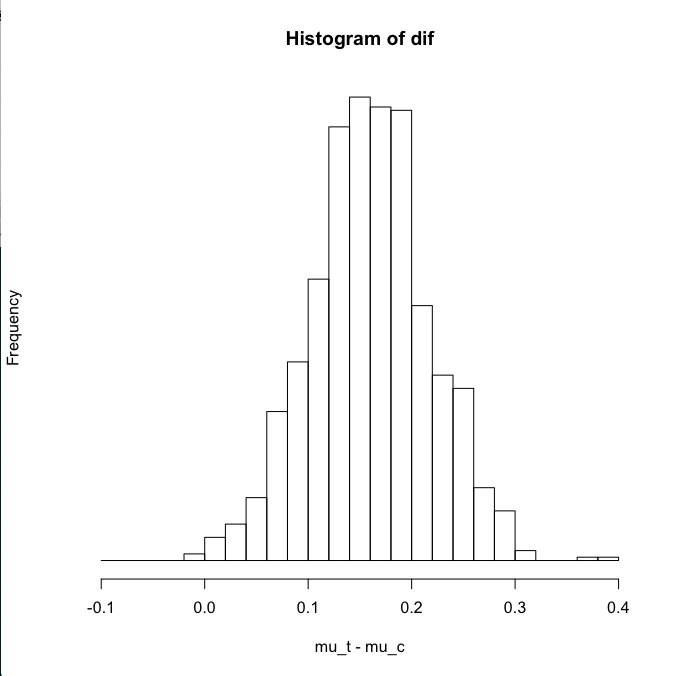
\includegraphics{question3.png}
  \caption{}
  \label{}
\end{figure}
\end{document}
